\documentclass[a4paper, 12pt]{article}

\usepackage[english,russian]{babel}
\usepackage[left=2cm, top=2cm, right=2cm, bottom=2.5cm]{geometry}
\usepackage{indentfirst}
\usepackage{enumitem}
\usepackage[tableposition=top,singlelinecheck=false]{caption}
\usepackage{subcaption}
\usepackage{graphicx}
\usepackage{wrapfig}
\usepackage{amssymb}
\usepackage{amsmath}
\usepackage{tabularx}

\setlist{nosep}

\DeclareCaptionLabelFormat{gostfigure}{\textbf{Рисунок #2}}
\DeclareCaptionLabelFormat{gosttable}{\textbf{Таблица #2}}
\DeclareCaptionLabelSeparator{gost}{.\;}
\captionsetup{labelsep=gost}
\captionsetup*[figure]{labelformat=gostfigure}
\captionsetup*[table]{labelformat=gosttable}
\renewcommand{\thesubfigure}{\asbuk{subfigure}}
\makeatletter
\newcommand*{\rom}[1]{\expandafter\@slowromancap\romannumeral #1@}
\makeatother

\begin{document}
    \pagenumbering{gobble}

\begin{center}
    {
        \MakeUppercase{Московский физико-технический институт}

        \MakeUppercase{(Национальный исследовательский университет)}
    }

    {
        Физтех-школа физики и исследований им. Ландау
    }
    
    \vspace{200pt}
    {
        \Huge
        \bfseries
        \MakeUppercase{Лабораторная работа №2.1.2}
    }

    \vspace{24pt}
    {
        \Large
        Определение показателя адиабаты методом изобарического расширения
    }

    \vspace{24pt}
    {
        \large
        Пилюгин Л.\,С.

        Б02-212
    }

    \vspace{2pt}
    {
        \large
        \today
    }
\end{center}

\newpage
\pagenumbering{arabic}
\setcounter{page}{2}

    \section{Аннотация}
\textbf{Цель работы:} применить методы обработки экспериментальных данный для
изучения статистических закономерностей при измерении интенсивности радиационного фона.

\textbf{Оборудование:} счётчик Гейгера-Мюллера (СТС-6), блок питания,
компьютер с интерфейсом связи со счётчиком.

    \section{Теоритические сведения}
\subsection{Распространение плоских монохроматических волн в одноосных кристаллах}
В некоторых кристаллах потенциальные ямы, в которых находятся электроны вблизи узлов решетки, не являются сферически симметричными. Для малых отклонений от положения равновесия потенциальная энергия электрона будет иметь вид
\[
    U  = a_{x}x^{2} + a_{y}y^{2} + q_{z}z^{2}
\]
Если $a_{y} = a_{z} = a_{\perp}$, $a_{x} = a_{\parallel}$, то кристалл называется одноосным с оптической осью $x$.

Так как одноосный кристалл неизотропен, векторы $\vec{E}$ и $\vec{D}$ в общем случае неколлинеарны:
\[
\vec{D} = \varepsilon_{\perp}\vec{E}_{\perp} + \varepsilon_{\parallel}\vec{E}_{\parallel}
\]

Распространение электромагнитных волн в отсутствие электрических зарядов и токов описывается уравнениями
\[
    \rot \vec{H} = \frac{1}{c}\frac{\partial \vec{D}}{\partial t}
\]
\[
    \rot \vec{E} = -\frac{1}{c}\frac{\partial\vec{H}}{\partial t}
\]
Плоские монохроматические волны в таких условиях описываются уравнениями
\[
    \vec{E} = \vec{E_{0}}\exp{\left(i\left(\omega t - \vec{k}\vec{r}\right)\right)}
\]
\[
    \vec{H} = \vec{H_{0}}\exp{\left(i\left(\omega t - \vec{k}\vec{r}\right)\right)}
\]
\[
    \vec{D} = \vec{D_{0}}\exp{\left(i\left(\omega t - \vec{k}\vec{r}\right)\right)}
\]
Отсюда следует, что $\rot\vec{H} = -i\vec{k}\times\vec{H}$, $\frac{\partial \vec{D}}{\partial t} = i \omega \vec{D}$ и аналогичные выражения для других векторов.

Подставив эти значения в уравнения Максвелла, получаем
\[
    \vec{D} = -\frac{c}{ \omega} \vec{k} \times \vec{H}
\]
\[
    \vec{H} = \frac{c}{ \omega} \vec{k} \times \vec{E}
\]

Отсюда видно, что $\vec{D}$, $\vec{H}$ и $\vec{k}$ взаимно перпендикулярны, а $\vec{E}$ лежит в одной плоскости с $\vec{D}$ и $\vec{k}$.

\begin{figure}[ht!]
    \center{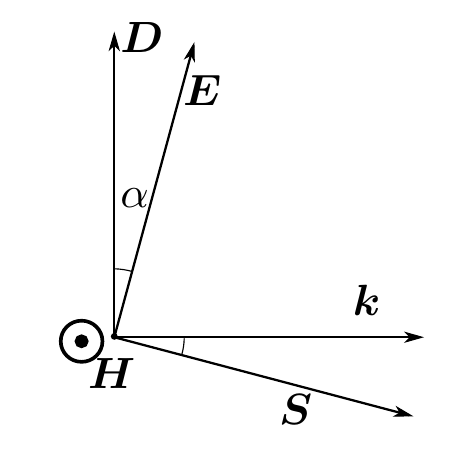
\includegraphics[width=0.4\linewidth]{../img/dehsk.png}}
\end{figure}

При этом выполнение материалистического уравнения возможно только если $\vec{D}$ перпендикулярен плоскости, в которой лежат оптическая ось кристалла и $\vec{k}$ (обыкновенная волна, рисунок слева), либо лежит в ней (необыкновенная волна, рисунок справа).

\begin{figure}[ht!]
    \center{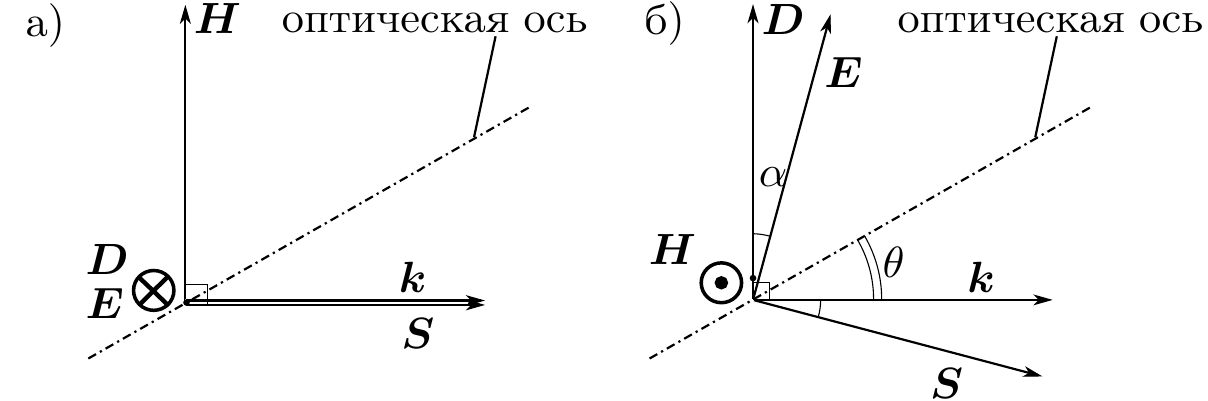
\includegraphics[width=0.8\linewidth]{../img/the.png}}
\end{figure}

Обыкновенная и необыкновенная волны распространяются в кристалле с разной скоростью. Обыкновенная волна поперечна относительно $\vec{E}$ и $\vec{H}$, поэтому для нее уравнения Максвелла те же, что и в изотропных средах, а скорость распространения
\[
    v_{\text{о}} = \frac{c}{\sqrt{ \varepsilon_{\perp}}} = \frac{c}{n_{\text{о}}}
\]
$n_{\text{о}} = \sqrt{ \varepsilon_{\perp}}$~--- коэффициент преломления обыкновенной волны.

Найдем фазовую скорость необыкновенной волны.
\[
    v = \frac{ \omega}{k} = \frac{cH}{D} = \frac{cE\cos \alpha}{H}, \text{См. рисунок и формулы связи $\vec{D}$, $\vec{E}$, $\vec{H}$ и $\vec{k}$}
\]
Исключая $H$ и выражая угол $ \alpha$ через скалярное произведение, получим
\[
    v = c\sqrt{\frac{E \cos \alpha}{D}} = c\sqrt{\frac{\vec{E} \vec{D}}{D^{2}}}
\]
\[
    \vec{E} \vec{D} = \varepsilon_{\parallel}E^{2}_{\parallel} + \varepsilon_{\perp}E^{2}_{\perp} = \frac{D_{\parallel}^{2}}{ \varepsilon_{\parallel}} + \frac{D_{\perp}^{2}}{ \varepsilon_{\perp}} = D^{2} \left(\frac{\sin^{2} \theta}{\varepsilon_{\parallel}} + \frac{\cos^{2} \theta}{ \varepsilon_{\perp}}\right)
\]

Получаем:
\[
    v_{\text{e}} = \frac{c}{n( \theta)}
\]
\[
n(\theta) = \frac{1}{\sqrt{\frac{\sin^{2} \theta}{ \varepsilon_{\parallel}} + \frac{\cos^{2} \theta}{ \varepsilon_{\perp}}}}
\]

Фазовая скорость необыкновенной волны зависит от угла между оптической осью и волновым вектором. Кроме того, вектор Поинтинга не коллинеарен волновому вектору, поэтому направление переноса энергии и переноса фазы не совпадают.

Плоская монохроматическая волна, попадающая из изотропной среды в одноосный кристалл, распадается на две взаимно ортогональные плоские волны, которые распространяются в разных направлениях и с разными скоростями.

\begin{figure}[ht!]
    \center{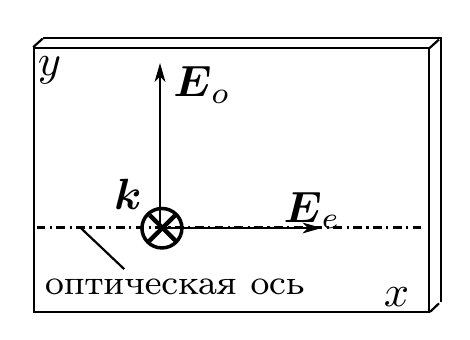
\includegraphics[width=0.4\linewidth]{../img/plast.png}}
\end{figure}
Важным частным случаем является распространение волн в одноосном кристалле перпендикулярно оптической оси. При этом у обыкновенной оси вектор $\vec{E}$ колеблется в плоскости, перпендикулярной этой оси. Для обыкновенной волны показатель преломления $n_{o} = \sqrt{ \varepsilon_{\perp}}$, а для необыкновенной $n_{e} = \sqrt{ \varepsilon_{\parallel}}$ (т.к. $ \theta = 90^{\circ}$).

Для нормально падающей волны компоненты обыкновенной и необыкновенной волн будут распространяться независимо и к моменту выхода наберут разность фаз
\[
    \Delta \varphi = kh\left(n_{e} - n_{o}\right)
\]

\subsection{Интерференция на одноосном кристалле}

Если перед одноосным кристаллом, помещенным между скрещенными поляроидами, поместить матовую пластинку, после которой лучи будут рассеиваться под разными углами, то на выходе образуется интерференционная картина в виде концентрических окружностей, перерезанных крестом. Эту картину образовали обыкновенные и необыкновенные лучи.

Коэффициент преломления для обыкновенного луча не зависит от угла падения на пластинку и равен $n_{1} = n_{o}$. Для необыкновенного луча в приближении малых углов $n_{2} = n_{o} - \left(n_{o} - n_{e}\right) \theta^{2}$. Таким образом разность фаз составляет
\[
    \Delta \varphi = \frac{2 \pi}{ \lambda} l \left(n_{o} - n_{e}\right) \theta^{2}
\]

Направлениями постояной разности фаз служат конусы. Из-за этого картина предствляет собой концентрические окружности. Крест выделяет те области, в которых распространяется только одна волна (обыкновенная или необыкновенная). При повороте выходного поляроида на $90^{\circ}$ картина меняется на противоположную.

Найдем радиус темного кольца $m$ в случае скрещенных поляроидов. При $m = 0$ сдвиг фаз равен нулю и луч не проходит анализатор. При сдвиге фаз $2\pi m$ ситуация аналогична. Поэтому
\[
    2\pi m = \frac{2\pi}{\lambda} l \left(n_{o} - n_{e}\right) \theta^{2}
\]
$\theta_{\text{внешн}} = n_{o}\theta$, поэтому
\[
    r_{m}^{2} = \frac{\lambda}{l} \frac{\left(n_{o}L\right)^{2}}{\left(n_{o} - n_{e}\right)} m
\]

\subsection{Влияние электрического поля}
Изотропное вещество можно превратить в неизотропное, поместив его в сильное электрическое поле. В этом случае электроны смещаются к новому положению равновесия и в потенциальной энергии появляются составляющие высоких порядков:
\[
    U = ax^{2} + \beta x^{3} + \gamma x^{4}
\]

Если $\beta \ne 0$, то вторая производная энергии окажется линейной функцией и получится эффект Поккельса: появится наведенное двулучепреломление, разность показателей преломления которого пропорциональна приложенному напряжению.

\begin{figure}[ht!]
    \center{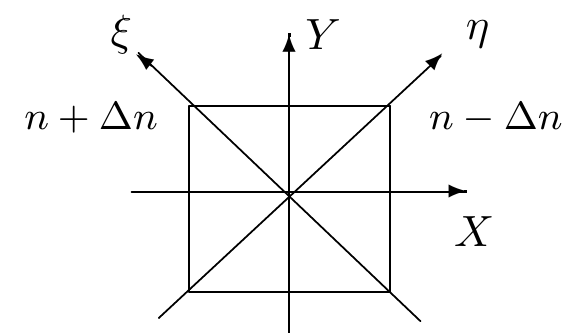
\includegraphics[width=0.5\linewidth]{../img/pok.png}}
\end{figure}

Поместим одноосный кристалл с осью $z$ в электрическое поле $E_{\text{эл}}$, направленное вдоль $x$. В данной работе свойства кристалла таковы, что в плоскости $xy$ появятся дополнительные перпендикулярные направления под углами $45^{\circ}$ к осям $x$ и $y$ с показателями преломления $n_{o} + \Delta n$ и $n_{o} + \Delta n$. Причем $\Delta n = A E_{\text{эл}}$. 

Пусть свет на входе в кристалл поляризован вертикально, а анализатор пропускает горизонтальную поляризацию. Разложим исходный вектор $E = E_{0} exp{\left(i\left(\omega t - kz\right)\right)}$ по осям $\xi$ и $\eta$. $E_{\xi} = E_{\eta} = E_{0} / \sqrt{2}$. После прохождения кристалла между векторами $E_{\xi}$ и $E_{\eta}$ появится разность фаз
\[
    \Delta \varphi = \frac{4\pi l}{\lambda}AE_{\text{эл}} = \frac{4\pi}{\lambda}\frac{l}{d}AU
\]
$U$~--- напряжение на кристалле, $d$~--- его поперечный размер.

Результирующее поле после анализатора~--- сумма проекций $E_{\xi}$ и $E_{\eta}$ на $x$:
\[
    E_{\text{вых}} = \frac{E_{0}}{2}\exp{\left(i\left(\omega t - kl\right)\right)}\left(e^{i\Delta \varphi / 2} - e^{-i\Delta\varphi / 2}\right) = E_{0}\exp{\left(i\left(\omega t - kr\right)\right)} \sin \left(\frac{ \Delta \varphi}{2}\right)
\]
В случае параллельных поляризаторов
\[
    E_{\text{вых}} =E_{0}\exp{\left(i\left(\omega t - kr\right)\right)} \cos \left(\frac{ \Delta \varphi}{2}\right) 
\]
Интенсивность света пропорциональна квадрату $E$. В случае скрещенных поляроидов:
\[
    I_{\text{вых}} = I_{0} \sin^{2} \left(\frac{ \Delta \varphi}{2}\right) = I_{0} \sin^{2} \left(\frac{\pi}{2}\frac{U}{U_{\lambda / 2}}\right) 
\]
В случае параллельных
\[
    I_{\text{вых}} = I_{0} \cos^{2} \left(\frac{\pi}{2}\frac{U}{U_{\lambda / 2}}\right)
\]

\[
    U_{\lambda /  2} = \frac{\lambda}{4A}\frac{d}{l}
\]
~--- полуволновое напряжение. При $U=U_{\lambda / 2}$ сдвиг фаз между двумя волнами равен $\pi$. 


    %\section{Оборудование}

    \section{Результаты измерений}
\subsection{Центровка элементов оптической системы}
\begin{tabular}{|c|c|c|c|c|}
\hline
    Линза & 1 & 2 & 3 & 4 \\\hline
    Приблизительное $F,\;\text{см}$ & $5$ -- $7$ & $15$ & $20$ & рассеивающая \\\hline
    $F,\;\text{см}$ & $7{,}7 \pm 0{,}1$ & $14{,}3 \pm 0{,}1$ & $19{,}5 \pm 0{,}1$ & $-8{,}5 \pm 1{,}4$ \\\hline
\end{tabular}

Для грубого определения фокусного расстояния получали изображение от лампы на поверхности стола и замеряли расстояние от линзы до поверхности. Та, которая не дала изображения~--- рассеивающая.

Для более точного определения фокусных расстояний поместили линзу 1 поместили так, чтобы она создавала параллельный пучок от источника (диафрагму почти полностью закрыли) и создавая точку на экране. Расстояние от линзы до экрана~--- фокусное.

\subsection{Определение фокусных расстояний при помощи экрана}
\begin{figure}[ht!]
    \center{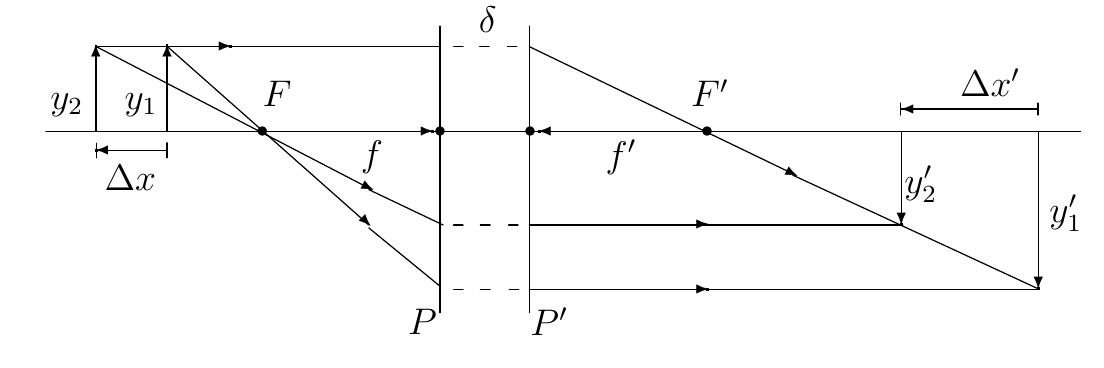
\includegraphics[width=0.8\linewidth]{../img/1.png}}
\end{figure}
Определим фокусное расстояние 1 линзы методом Аббе. $y_{1} = y_{2} = 2{,}0\pm 0{,}05\;\text{см}$.

\begin{tabular}{|c|c|c|}
\hline
     & 1 & 2 \\\hline
    $f,\pm 0{,}5\;\text{см}$ & $17$ & $42{,}5$ \\\hline
    $d,\pm 0{,}5\;\text{см}$  & $12{,}5$ & $9{,}5$ \\\hline
    $y',\pm 0{,}05\;\text{см}$ & $2{,}7$ & $8{,}9$ \\\hline
\end{tabular}

$\Delta x = d_{2} - d_{1} = -3\pm 1\;\text{см}$
$\Delta x' = f_{2} - f_{1} = 25\pm 1\;\text{см}$
$F_{1} = \frac{\Delta x}{y_{1} / y_{1}' - y_{2}/y_{2}'} = 5\pm 2\;\text{см}$
$F_{2} = \frac{\Delta x'}{y_{1}' / y_{1} - y_{2}' / y_{2}} = 8{,}0 \pm 0{,}4\;\text{см}$.

Полученные фокусные расстояния для первой линзы заметно отличаются друг от друга. Это может быть связано с неточностями в измерении расстояний от предмета до линзы и от линзы до изображения.

\begin{figure}[ht!]
    \center{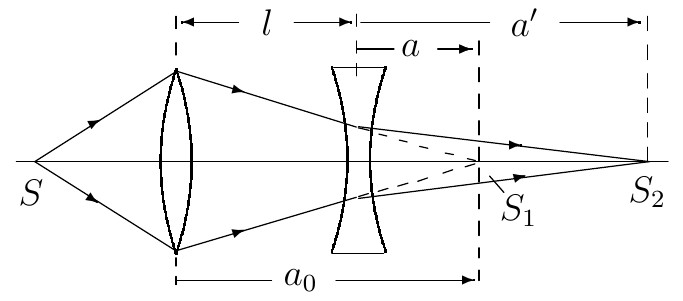
\includegraphics[width=0.8\linewidth]{../img/2.png}}
\end{figure}
Для определения фокусного расстояния рассеивающей линзы соберем схему, изображенную на рисунке.
$a_{0} = 44{,}5 \pm 0{,}5\;\text{см}$, $a' = 19{,}5 \pm 0{,}5 \;\text{см}$, $l = 38{,}5 \pm 0{,}5 \;\text{см}$.
\[
    \frac{1}{F} = -\frac{1}{a_{0} - l} + \frac{1}{a'}
\]
$F = -8{,}5 \pm 1{,}4\;\text{см}$

\subsection{Определение фокусного расстояния и положения главных и фокальных плоскостей сложной оптической системы}

$l_{12} = 5\pm 0{,}1\;\text{см}$, $l_{2} = 3{,}5 \pm 0{,}1\;\text{см}$, $l_{1} = 10{,}3 \pm 0{,}1 \;\text{см}$, $y_{1}' = 5,0 \pm 0{,}1\;\text{см}$, $y_{2}' = 1{,}4 \pm 0{,}1 \;\text{см}$, $x_{1} = 25{,}5 \pm 0{,}1 \;\text{см}$, $x_{2} = 13{,}4 \pm 0{,}1\;\text{см}$.

$\Delta x = -6{,}8 \pm 0{,}2 \;\text{см}$, $\Delta x' = -12{,}1 \pm 0{,}2 \;\text{см}$.

\[
    F_{1} = \frac{\Delta x}{y_{1} / y_{1}' - y_{2} / y_{2}'} =  6{,}6 \pm 0{,}4\;\text{см}
\]
\[
    F_{2} = \frac{\Delta x'}{y_{2}' / y_{2} - y_{1}' / y_{1}} = 6{,}7 \pm 0{,}4\;\text{см} 
\]
\[
    \frac{1}{F_{3}} = \frac{1}{F_{1}} + \frac{1}{F_{2}} - \frac{l_{12}}{F_{1}F_{2}}
\]
\[
    F_{3} = 6{,}5 \pm 0{,}2\;\text{см}
\]

Пункт 14 выполнялся для линз 2 и 3, т.к. линзы 1 и 2 давали слишком большую оптическую силу.
$x_{1} = 6 \pm 0{,}1\;\text{см}$.
В обратную сторону пустить луч не получилось из-за выступающего винта регулировки линзы 3.

    \section{Вывод}
Была снята зависимость коэффициента поверхностного натяжения воды от температуры.
Результаты (за исключением двух выбросных точек) с учетом погрешности согласуются
с табличными значениями.
\end{document}
